%%%%%%%%%%%%%%%%%%%%%%%%%%%%%%%%%%%%%%%%%%
% Mathematics Final Year Research Projects
% LaTeX Template
% Version 1.0 (31/01/24)
%
% This template has been adapted from: https://www.overleaf.com/latex/templates/imperial-college-report-template/wncnzptkhnbc
% Students should feel free to adapt this template to their needs.
%%%%%%%%%%%%%%%%%%%%%%%%%%%%%%%%%%%%%%%%%%
%----------------------------------------------------------------------------------------
% PACKAGES AND OTHER DOCUMENT CONFIGURATIONS
%----------------------------------------------------------------------------------------
\documentclass[a4paper,11pt, twoside]{report}

%% Language and font encodings
\usepackage[english]{babel}
\usepackage[utf8]{inputenc}
\usepackage[T1]{fontenc}

%% Imperial Recommended Packages
\usepackage{afterpage}

% Lean colour configurations
\usepackage{color}
\definecolor{keywordcolor}{rgb}{0.7, 0.1, 0.1}   % red
\definecolor{tacticcolor}{rgb}{0.0, 0.1, 0.6}    % blue
\definecolor{commentcolor}{rgb}{0.4, 0.4, 0.4}   % grey
\definecolor{symbolcolor}{rgb}{0.0, 0.1, 0.6}    % blue
\definecolor{sortcolor}{rgb}{0.1, 0.5, 0.1}      % green
\definecolor{attributecolor}{rgb}{0.7, 0.1, 0.1} % red
\definecolor{backcolour}{rgb}{0.95,0.95,0.92}

% Listings (for displaying code):
\usepackage{listings}
\def\lstlanguagefiles{TeX_Setup/lstlean.tex}
\lstset{
    % frame = single, 
    % framexleftmargin=15pt,
    language = lean,
    numbers = left,
    backgroundcolor=\color{backcolour}
}

% ----------- Algorithm2e setup
\usepackage[ruled,vlined]{algorithm2e}
\makeatletter
\renewcommand{\SetKwInOut}[2]{%
  \sbox\algocf@inoutbox{\KwSty{#2}\algocf@typo:}%
  \expandafter\ifx\csname InOutSizeDefined\endcsname\relax% if first time used
    \newcommand\InOutSizeDefined{}\setlength{\inoutsize}{\wd\algocf@inoutbox}%
    \sbox\algocf@inoutbox{\parbox[t]{\inoutsize}{\KwSty{#2}\algocf@typo:\hfill}~}\setlength{\inoutindent}{\wd\algocf@inoutbox}%
  \else% else keep the larger dimension
    \ifdim\wd\algocf@inoutbox>\inoutsize%
    \setlength{\inoutsize}{\wd\algocf@inoutbox}%
    \sbox\algocf@inoutbox{\parbox[t]{\inoutsize}{\KwSty{#2}\algocf@typo:\hfill}~}\setlength{\inoutindent}{\wd\algocf@inoutbox}%
    \fi%
  \fi% the dimension of the box is now defined.
  \algocf@newcommand{#1}[1]{%
    \ifthenelse{\boolean{algocf@inoutnumbered}}{\relax}{\everypar={\relax}}%
%     {\let\\\algocf@newinout\hangindent=\wd\algocf@inoutbox\hangafter=1\parbox[t]{\inoutsize}{\KwSty{#2}\algocf@typo\hfill:}~##1\par}%
    {\let\\\algocf@newinout\hangindent=\inoutindent\hangafter=1\parbox[t]{\inoutsize}{\KwSty{#2}\algocf@typo:\hfill}~##1\par}%
    \algocf@linesnumbered% reset the numbering of the lines
  }}%
\makeatother
% --------- end algorithm2e setup

\usepackage{bm}
\usepackage[normalem]{ulem}

\usepackage[colorinlistoftodos]{todonotes}

% I have all of their other recommended packages somewhere on here.

\usepackage[most]{tcolorbox}
\usepackage{authblk}  % Lets you add an \affil{} to your title, stating your affiliation {eg. Sigma Mathematics Society}
\usepackage{ragged2e}
\usepackage{csquotes}
\usepackage{pdfpages}



\usepackage{xfrac}
\usepackage{cancel}

\usepackage[inline]{enumitem}

%\usepackage{tgpagella}

\usepackage{blindtext}
\usepackage{lipsum}
\usepackage{verbatim}
\usepackage{hyperref}
\hypersetup{
    citebordercolor = 1 1 1,
    linkbordercolor = 1 1 1,
    filebordercolor = 1 1 1,
    menubordercolor = 1 1 1,
    urlbordercolor = 1 1 1,
    colorlinks  =   true,
    linkcolor   =   blue,
    citecolor   =   magenta,
    urlcolor    =   blue
}

% This project uses natbib instead. See end of format file.
% \usepackage{biblatex} % Modify citation format using [style=yourstyle] parameter--eg \usepackage[style=mla-new]{biblatex}
% \bibliography{TeX_Setup/References.bib}
% \addbibresource{TeX_Setup/References.bib}

\usepackage{cancel}
\usepackage{amssymb}
\usepackage{amsmath}
% \usepackage{amsthm}  % In `environments.tex`
%\usepackage{MnSymbol}
\usepackage{mathrsfs}
\usepackage{mathtools}
% \usepackage{mathabx}
\usepackage{mathdots}
\usepackage{yhmath}

\usepackage{array}
\usepackage{booktabs}
\usepackage{longtable}

\usepackage{graphicx}
\newcommand\sbullet[1][.5]{\mathbin{\vcenter{\hbox{\scalebox{#1}{$\bullet$}}}}}  % Bullet of customisable size
\usepackage{wrapfig}
% Imperial-recommended `caption` setup
\usepackage{caption}
\captionsetup[figure]{labelfont={bf}, name={Figure}, justification=centering}
\captionsetup[table]{labelfont={bf}, name={Table}}
\usepackage{subcaption}
\usepackage{tikz}
\usepackage{float}

% Tikz
\usepackage{tikz-cd}
\usepackage{tikz-3dplot}
\usetikzlibrary{positioning}
\usetikzlibrary{cd}
\usetikzlibrary{shapes.geometric}
\usepackage{pgfplots}
\usepackage{mathrsfs}
\usetikzlibrary{arrows}
\usepackage{qtree}

%% Sets page size and margins
\usepackage[a4paper,top=1in,bottom=1in,left=1in,right=1in,marginparwidth=1.75cm]{geometry}

% Font

% \usepackage{sansmathfonts}
% % \usepackage{mathrsfs}
% \usepackage[T1]{fontenc}
% \renewcommand*\familydefault{\sfdefault}

\renewcommand*{\rmdefault}{bch}
\renewcommand*{\ttdefault}{lmtt}

% Structure and Numbering

\usepackage{fancyhdr}
\usepackage{lastpage}

\pagestyle{fancy}
\fancyhf{}

\rhead{{Page \thepage}}%\hspace{1pt} of \pageref{LastPage}}}
\lhead{\textit\slshape\nouppercase{\leftmark}}

\numberwithin{equation}{section}

% Lists

\setlist[description]{font=\normalfont}
\setlist[enumerate]{before=\normalfont}

% Spacing and indentation

% Not sure if 1.5-spacing is permitted. I'll leave it commented out for now.
% \usepackage{setspace}
% \renewcommand{\baselinestretch}{1.5}

\usepackage[skip=11pt, indent=0pt]{parskip}
% Here's what Imperial's recommended setup is:
% \setlength{\parskip}{0.5em}
% \usepackage{indentfirst}  % Uncomment if using above

\allowdisplaybreaks  % Allows align environments to continue for several pages

% Colours

\usepackage{xcolor}
\definecolor{darkblue}{rgb}{0.0, 0.0, 0.55}
\definecolor{pink}{rgb}{0.858, 0.188, 0.478}
\definecolor{brown}{rgb}{0.8, 0.4, 0.0}

% Bibliography
\usepackage[numbers, comma, square, sort&compress]{natbib}
\bibliographystyle{References/abbrvunsrtnat.bst}
% \bibliographystyle{unsrtnat}

\usepackage{amsthm}
% Gives theorem and definition names the same font style as the words "theorem"/"definition": see https://tex.stackexchange.com/questions/43966/how-to-make-the-optional-title-of-a-theorem-bold-with-amsthm
\makeatletter
\def\th@plain{%
  \thm@notefont{}% same as heading font
  \itshape % body font
}
\def\th@definition{%
  \thm@notefont{}% same as heading font
  \normalfont % body font
}
\makeatother

\usepackage{cleveref}

\newtheorem*{theorem*}{Theorem}
\newtheorem{theorem}{Theorem}[section]
\newtheorem{corollary}[theorem]{Corollary}%[theorem]
\newtheorem{lemma}[theorem]{Lemma}
\newtheorem{claim}[theorem]{Claim}
\newtheorem{conjecture}[theorem]{Conjecture}
% \newtheorem{algorithm}[theorem]{Algorithm}  % Defined in algorithm2e
\newtheorem{proposition}[theorem]{Proposition}

\newtheorem{problem}[theorem]{Problem}
\newenvironment{boxproblem}{
    \begin{tcolorbox}[colback=yellow!15!white,colframe=orange, breakable, enhanced]\begin{problem}
}{
    \end{problem}\end{tcolorbox}
}

\newenvironment{boxtheorem}{
    \begin{tcolorbox}[colback=yellow!15!white,colframe=orange, breakable, enhanced]\begin{theorem}
}{
    \end{theorem}\end{tcolorbox}
}
\newenvironment{boxproposition}{
    \begin{tcolorbox}[colback=yellow!15!white,colframe=orange, breakable, enhanced]\begin{proposition}
}{
    \end{proposition}\end{tcolorbox}
}
\newenvironment{boxlemma}{
    \begin{tcolorbox}[colback=yellow!15!white,colframe=orange, breakable, enhanced]\begin{lemma}
}{
    \end{lemma}\end{tcolorbox}
}
\newenvironment{boxcorollary}{
    \begin{tcolorbox}[colback=yellow!15!white,colframe=orange, breakable, enhanced]\begin{corollary}
}{
    \end{corollary}\end{tcolorbox}
}
\newenvironment{boxconjecture}{
    \begin{tcolorbox}[colback=yellow!15!white,colframe=orange, breakable, enhanced]\begin{conjecture}
}{
    \end{conjecture}\end{tcolorbox}
}


\theoremstyle{remark}
\newtheorem*{remark}{Remark}
\newtheorem*{solution}{Solution}

\theoremstyle{definition}
\newtheorem{definition}[theorem]{Definition}
\newenvironment{boxdefinition}{
    \begin{tcolorbox}[colback=cyan!10!white,colframe=cyan!70!black, breakable, enhanced]\begin{definition}
}{
    \end{definition}\end{tcolorbox}
}
\newtheorem*{convention}{Convention}
\newenvironment{boxconvention}{
    \begin{tcolorbox}[colback=magenta!3!white,colframe=magenta!70!black, breakable, enhanced]\begin{convention}
}{
    \end{convention}\end{tcolorbox}
}
\newtheorem*{notation}{Notation}
\newenvironment{boxnotation}{
    \begin{tcolorbox}[colback=magenta!3!white,colframe=magenta!70!black, breakable, enhanced]\begin{notation}
}{
    \end{notation}\end{tcolorbox}
}
\newtheorem{example}[theorem]{Example}
\newenvironment{boxexample}{
    \begin{tcolorbox}[colframe=green!30!black, breakable, enhanced, breakable, enhanced]\begin{example}
}{
    \end{example}\end{tcolorbox}
}
\newtheorem{nexample}[theorem]{Non-Example}
\newenvironment{boxnexample}{
    \begin{tcolorbox}[colframe=red!50!black, breakable, enhanced]\begin{nexample}
}{
    \end{nexample}\end{tcolorbox}
}
\newtheorem{cexample}[theorem]{Counterexample}
\newenvironment{boxcexample}{
    \begin{tcolorbox}[colframe=red!50!black, breakable, enhanced]\begin{cexample}
}{
    \end{cexample}\end{tcolorbox}
}

% \def\SMALLCOLWIDTH{1.5cm}
\newcolumntype{C}[1]{>{\centering\let\newline\\\arraybackslash\hspace{0pt}}m{#1}}

% Centering captions
% \renewcommand{\caption}[1]{\caption{\centering #1}}

%%%%%%%%%%%%%%%%%%%%%%%%%%%%%%%%%%%%%%%%%%%%%%%%%%%%%%%%%%%%%%%%%%%%%%%%%%%%%%%%%%%%%%%%%%%%%%%%%%%%%%%%%%%%
% CUSTOM COMMANDS
%%%%%%%%%%%%%%%%%%%%%%%%%%%%%%%%%%%%%%%%%%%%%%%%%%%%%%%%%%%%%%%%%%%%%%%%%%%%%%%%%%%%%%%%%%%%%%%%%%%%%%%%%%%%

% Custom colours

\definecolor{darkgreen}{rgb}{0.1, 0.4, 0.3}      % green

% `sorry`

\newcommand{\sorry}{\textcolor{red}{\texttt{sorry}}}
% \newcommand{\sorry}{\lstinline{sorry}}

% TIKZ:

\newcommand{\drawplane}{  % For use with TikZ
    \draw[step=0.5cm,gray,very thin] (-2.5,-2.5) grid (2.5,2.5);
    \draw[thick,->] (-2.5,0) -- (2.5,0); % node[anchor=west] {$x$};
    \draw[thick,->] (0,-2.5) -- (0,2.5); % node[anchor=south] {$y$};
    % \node[black, anchor=north east] at (0, 0) {$0$};
}
\newcommand{\latticecircle}[2]{
    \draw[fill=yellow, opacity=0.5] (#1, #2) circle (0.5);
    \node at (#1, #2) {\color{gray}{$\bullet$}};
}
\newcommand{\latticecirclegrey}[2]{
    \draw[fill=gray, opacity=0.75] (#1, #2) circle (0.5);
    \node at (#1, #2) {\color{black}{$\bullet$}};
}
\newcommand{\latticecirclebrown}[2]{
    \draw[fill=brown, opacity=0.75] (#1, #2) circle (0.5);
    \node at (#1, #2) {\color{black}{$\bullet$}};
}
\usetikzlibrary{decorations.markings}
\tikzset{->-/.style={decoration={
      markings,
      mark=at position #1 with {\arrow{>}}},postaction={decorate}
}}

\newenvironment{cd}{
    \begin{equation} \begin{tikzcd}
}{
    \end{tikzcd} \end{equation}
}
\newenvironment{cd*}{
    \begin{equation*} \begin{tikzcd}
}{
    \end{tikzcd} \end{equation*}
}

\newcommand{\drawsquare}[1]{
    \draw[thick, blue]
    (-{#1},-{#1}) node [anchor=north east] {C} --
    (-{#1}, {#1}) node[anchor=south east] {B} --
    ({#1}, {#1}) node[anchor=south west] {A} --
    ({#1}, -{#1}) node [anchor=north west] {D} -- cycle;
}

\newcommand{\labelledpoint}[5]{ % Takes x coord, y coord, label x-position relative to point, label y-position relative to point, label text as arguments
    \node [label={[shift={(#3,#4)}]#5}] at (#1, #2) {$\bullet$};
}

% DELIMITERS:

\newcommand{\parenth}[1]{\left( #1 \right)}
\newcommand{\brac}[1]{\left[ #1 \right]}
\newcommand{\set}[1]{\left\{ #1 \right\}}
\newcommand{\setst}[2]{\set{#1 \; \middle\vert \; #2}}
\newcommand{\abs}[1]{\left\lvert #1 \right\rvert}
\newcommand{\norm}[1]{\left\lVert #1 \right\rVert}
\newcommand{\floor}[1]{\left\lfloor #1 \right\rfloor}
\newcommand{\ceil}[1]{\left\lceil #1 \right\rceil}
\newcommand{\cycl}[1]{\left\langle #1 \right\rangle}
\newcommand{\grpres}[2]{\cycl{#1 \; \middle| \; #2}}  % \grpres{gens}{rels}

% FUNCTIONS:

\newcommand{\fx}{f\!\parenth{x}}
\newcommand{\fof}[1]{f\!\parenth{#1}}

\newcommand{\px}{p\!\parenth{x}}
\newcommand{\pof}[1]{p\!\parenth{#1}}
\newcommand{\pofbig}[1]{p\Big(#1\Big)}
\newcommand{\gx}{g\!\parenth{x}}
\newcommand{\gof}[1]{g\!\parenth{#1}}
\newcommand{\hx}{h\!\parenth{x}}
\newcommand{\hof}[1]{h\!\parenth{#1}}
\newcommand{\Tv}{T\!\parenth{v}}
\newcommand{\Tof}[1]{T\!\parenth{#1}}
\newcommand{\Tbar}{\overline{T}}
\newcommand{\Tbarof}[1]{\Tbar\!\parenth{#1}}
\newcommand{\Tbarv}{\Tbarof{v}}
\newcommand{\Sof}[1]{S\!\parenth{#1}}

\newcommand{\psin}[1]{\sin\!{\parenth{#1}}}
\newcommand{\pcos}[1]{\cos\!{\parenth{#1}}}
\newcommand{\ptan}[1]{\tan\!{\parenth{#1}}}
\newcommand{\sinsq}[1]{\sin^2\!\parenth{#1}}
\newcommand{\cossq}[1]{\cos^2\!\parenth{#1}}
\newcommand{\tansq}[1]{\tan^2\!\parenth{#1}}
\newcommand{\parcsin}[1]{\arcsin\!{\parenth{#1}}}
\newcommand{\parccos}[1]{\arccos\!{\parenth{#1}}}
\newcommand{\parctan}[1]{\arctan\!{\parenth{#1}}}

\newcommand{\logbase}[2]{\log_{#1}\!\parenth{#2}}
\newcommand{\nthroot}[2]{\sqrt[\leftroot{-3}\uproot{3} #1]{#2}}
\newcommand{\cbrt}[1]{\nthroot{3}{#1}}

\newcommand{\pgcd}[2]{\gcd\!\parenth{{#1},{#2}}}
\newcommand{\plcm}[2]{\operatorname{lcm}\!\parenth{{#1},{#2}}}
\newcommand{\pgcds}[1]{\gcd\!\parenth{#1}}
\newcommand{\plcms}[1]{\operatorname{lcm}\!\parenth{#1}}

\newcommand{\varphiof}[1]{\varphi\!\parenth{#1}}
\newcommand{\phiof}[1]{\phi\!\parenth{#1}}
\newcommand{\xiof}[1]{\xi\!\parenth{#1}}
\newcommand{\rhoof}[1]{\rho\!\parenth{#1}}
\newcommand{\pexp}[1]{\exp\!\parenth{#1}}

\newcommand{\inj}{\hookrightarrow}
\newcommand{\surj}{\twoheadrightarrow}

\DeclareMathOperator*{\argmin}{\arg\!\min}
\DeclareMathOperator*{\argmax}{\arg\!\max}

\newcommand{\of}[1]{\!\parenth{#1}}

% CALCULUS:

\newcommand{\dx}{\operatorname{d}\!x}
\newcommand{\dy}{\operatorname{d}\!y}
\newcommand{\diff}[1]{\operatorname{d}\!{#1}}
\newcommand{\dydx}{\frac{\dy}{\dx}}

% LINEAR ALGEBRA:

\newcommand{\mat}[3]{\operatorname{M}_{{#1} \times {#2}}\!\parenth{{#3}}}
\newcommand{\matsq}[2]{\operatorname{M}_{{#1} \times {#1}}\!\parenth{\mathbb{#2}}}
\newcommand{\MnR}{\operatorname{M}_{n}\!\parenth{\real}}
\newcommand{\MnC}{\operatorname{M}_{n}\!\parenth{\C}}
\newcommand{\Mn}[2]{\operatorname{M}_{#1}\!\parenth{#2}}
\newcommand{\GL}[1]{\operatorname{GL}\!\parenth{#1}}
\newcommand{\SL}[1]{\operatorname{SL}\!\parenth{#1}}
\newcommand{\PGL}[1]{\operatorname{PGL}\!\parenth{#1}}
\newcommand{\PSL}[1]{\operatorname{PSL}\!\parenth{#1}}

\newcommand{\Span}[1]{\operatorname{Span}\!\parenth{#1}}

\newcommand{\pdim}[1]{\dim\!\parenth{#1}}

\newcommand{\RSp}[1]{\operatorname{RSp}\!\parenth{#1}}
\newcommand{\CSp}[1]{\operatorname{CSp}\!\parenth{#1}}
\newcommand{\rank}[1]{\operatorname{rank}\!\parenth{#1}}
\newcommand{\pim}[1]{\operatorname{im}\!\parenth{#1}}
\newcommand{\pker}[1]{\operatorname{ker}\!\parenth{#1}}
\newcommand{\pdet}[1]{\det\!\parenth{#1}}

\newcommand{\cA}[1]{c_A \! \parenth{#1}}
\newcommand{\cB}[1]{c_B \! \parenth{#1}}
\newcommand{\mA}[1]{m_A \! \parenth{#1}}
\newcommand{\mB}[1]{m_B \! \parenth{#1}}
\newcommand{\cAx}{\cA{x}}
\newcommand{\cBx}{\cB{x}}
\newcommand{\mAx}{\mA{x}}
\newcommand{\mBx}{\mB{x}}
\newcommand{\cof}[2]{c_{#1}\!\parenth{#2}}
\newcommand{\mof}[2]{m_{#1}\!\parenth{#2}}

\newcommand{\Cof}[1]{C\!\parenth{#1}}
\newcommand{\+}{\oplus}
\newcommand{\pdeg}[1]{\deg\!\parenth{#1}}

\newcommand{\RCF}[1]{\operatorname{RCF}\!\parenth{#1}}
\newcommand{\JCF}[1]{\operatorname{JCF}\!\parenth{#1}}

\newcommand{\Jsub}[2]{J_{#1}\!\parenth{#2}}

\newcommand{\Aof}[1]{A\!\parenth{#1}}

\newcommand{\Tsub}[2]{T_{#1}\!\parenth{#2}}

\newcommand{\Tr}[1]{\operatorname{Tr}\!\parenth{#1}}

\newcommand{\diag}[1]{\operatorname{diag}\!\parenth{#1}}

% Measure Theory

\newcommand{\muof}[1]{\mu\!\parenth{#1}}
\newcommand{\muA}{\muof{A}}
\newcommand{\muB}{\muof{B}}
\newcommand{\mutof}[1]{\Tilde{\mu}\!\parenth{#1}}
\newcommand{\mustof}[1]{\mu^*\!\parenth{#1}}
\newcommand{\calF}{\mathcal{F}}
\newcommand{\calA}{\mathcal{A}}
\newcommand{\calB}{\mathcal{B}}
\newcommand{\calC}{\mathcal{C}}
\newcommand{\sigmaof}[1]{\sigma\!\parenth{#1}}
\newcommand{\psiof}[1]{\psi\!\parenth{#1}}

% Intervals

\newcommand{\Ioc}[1]{\left(#1\right]}
\newcommand{\Ico}[1]{\left[#1\right)}

% GROUPS/ALGEBRA IN GENERAL:

\newcommand{\inv}{^{-1}}
\newcommand{\Sym}[1]{\operatorname{Sym}\!\parenth{#1}}
\newcommand{\ord}[1]{\operatorname{ord}\!\parenth{#1}}
\newcommand{\supp}[1]{\operatorname{supp}\!\parenth{#1}}
\newcommand{\sgn}[1]{\operatorname{sgn}\!\parenth{#1}}
\newcommand{\tcyc}[2]{\begin{pmatrix} #1 & #2 \end{pmatrix}}

\newcommand{\nsg}{\trianglelefteq}

\newcommand{\Rmul}{R^{\times}}
\newcommand{\kmul}{k^{\times}}
\newcommand{\kX}{k\!\brac{X}}
\newcommand{\RX}{R\!\brac{X}}

\newcommand{\quotient}[2]{
    \left.\raisebox{.2em}{${#1}$} \middle/ \raisebox{-.2em}{${#2}$} \right.
}
\newcommand{\Zmod}[1]{\quotient{\Z}{{#1}\Z}}

\newcommand{\Vof}[1]{V\!\parenth{#1}}

\newcommand{\Frac}[1]{\operatorname{Frac}\!\parenth{#1}}

\newcommand{\Spec}[1]{\operatorname{Spec}\!\parenth{#1}}

\newcommand{\id}{\operatorname{id}}

\newcommand{\pchar}[1]{\operatorname{char}\!\parenth{#1}}

\newcommand{\Hom}{\operatorname{Hom}}

\newcommand{\Zof}[1]{\operatorname{Z}\!\parenth{#1}}

\newcommand{\Aut}[1]{\operatorname{Aut}\!\parenth{#1}}

% NUMBER SETS:

\newcommand{\real}{\mathbb{R}}
\newcommand{\rational}{\mathbb{Q}}
\newcommand{\naturalnum}{\mathbb{N}}
\newcommand{\integers}{\mathbb{Z}}
\newcommand{\complex}{\mathbb{C}}

\newcommand{\Field}{\mathbb{F}}
\newcommand{\Q}{\mathbb{Q}}
\newcommand{\R}{\real}
\newcommand{\N}{\naturalnum}
\newcommand{\Z}{\integers}
\newcommand{\C}{\complex}
\newcommand{\B}{\mathcal{B}}
\newcommand{\I}{\mathcal{I}}
\newcommand{\J}{\mathcal{J}}

\newcommand{\psup}[1]{\sup\!\parenth{#1}}
\newcommand{\pinf}[1]{\inf\!\parenth{#1}}

% LOGIC:

\newcommand{\ergo}{\therefore}
\newcommand{\bcos}{\because}
\newcommand{\st}{\text{ s.t. }}


% -------------------- SPECIFIC TO PROJECT -------------------- %

% TERMINOLOGY

\newcommand{\CELP}{Cohn-Elkies Linear Programming Bound}
\newcommand{\CEC}{Cohn-Elkies Conditions}
\newcommand{\JCT}{Jordan Curve Theorem}
\newcommand{\CGT}{Cauchy-Goursat Theorem}

% NOTATION

\newcommand{\Pa}{\mathcal{P}}
\newcommand{\Vol}{\operatorname{Vol}}
\newcommand{\Volof}[1]{\Vol\!\parenth{#1}}
\newcommand{\Sch}{\mathcal{S}}
\renewcommand{\hat}{\widehat}
\renewcommand{\tilde}{\widetilde}
\newcommand{\F}{\mathcal{F}}
\newcommand{\periodic}{\operatorname{periodic}}

\newcommand{\Halfplane}{\mathbb{H}} % Using Lean notation for the upper-half plane instead of Viazovska's

\newcommand{\BigO}[1]{\operatorname{O}\of{#1}}

\newcommand{\fm}{f \mid}
\newcommand{\fmof}[3]{\parenth{\fm_{#1} {#2}}\of{#3}}

% COMPLEX ANALYSIS

\renewcommand{\Re}{\operatorname{Re}}
\renewcommand{\Im}{\operatorname{Im}}

\newcommand{\rad}{_{\operatorname{rad}}}

% LEAN

\newcommand{\mathlib}{\texttt{mathlib}}


% %% Useful packages
% \usepackage{afterpage}
% \usepackage{amsmath}
% \usepackage{amsthm}
% \usepackage{amssymb}
% \usepackage{csquotes}
% \usepackage{enumitem}
% \usepackage{graphicx}
% \usepackage{lipsum}
% \usepackage{booktabs}

% % Listings (for displaying code):
% \usepackage{listings}
% \lstset{
%     frame = single, 
%     framexleftmargin=15pt
% }

% % Center figure captions:
% \usepackage{caption}
% \captionsetup[figure]{labelfont={bf},name={Figure},labelsep=quad}
% \captionsetup[table]{labelfont={bf},name={Table},labelsep=quad}


% % ----------- Algorithm2e setup
% \usepackage[ruled,vlined]{algorithm2e}
% \makeatletter
% \renewcommand{\SetKwInOut}[2]{%
%   \sbox\algocf@inoutbox{\KwSty{#2}\algocf@typo:}%
%   \expandafter\ifx\csname InOutSizeDefined\endcsname\relax% if first time used
%     \newcommand\InOutSizeDefined{}\setlength{\inoutsize}{\wd\algocf@inoutbox}%
%     \sbox\algocf@inoutbox{\parbox[t]{\inoutsize}{\KwSty{#2}\algocf@typo:\hfill}~}\setlength{\inoutindent}{\wd\algocf@inoutbox}%
%   \else% else keep the larger dimension
%     \ifdim\wd\algocf@inoutbox>\inoutsize%
%     \setlength{\inoutsize}{\wd\algocf@inoutbox}%
%     \sbox\algocf@inoutbox{\parbox[t]{\inoutsize}{\KwSty{#2}\algocf@typo:\hfill}~}\setlength{\inoutindent}{\wd\algocf@inoutbox}%
%     \fi%
%   \fi% the dimension of the box is now defined.
%   \algocf@newcommand{#1}[1]{%
%     \ifthenelse{\boolean{algocf@inoutnumbered}}{\relax}{\everypar={\relax}}%
% %     {\let\\\algocf@newinout\hangindent=\wd\algocf@inoutbox\hangafter=1\parbox[t]{\inoutsize}{\KwSty{#2}\algocf@typo\hfill:}~##1\par}%
%     {\let\\\algocf@newinout\hangindent=\inoutindent\hangafter=1\parbox[t]{\inoutsize}{\KwSty{#2}\algocf@typo:\hfill}~##1\par}%
%     \algocf@linesnumbered% reset the numbering of the lines
%   }}%
% \makeatother
% % --------- end algorithm2e setup

% % \bm allows typing bold math:
% \usepackage{bm}
% \usepackage[normalem]{ulem}

% \usepackage[colorinlistoftodos]{todonotes}
% \usepackage[colorlinks=true, allcolors=blue]{hyperref}

% \renewcommand*{\rmdefault}{bch}
% \renewcommand*{\ttdefault}{lmtt}
% \newcommand{\citationneeded}{\textcolor{red}{[citation-needed]}}

% % Add bigger skip between paragraphs, makes reading easier:
% \setlength{\parskip}{0.5em}

% % Bibliography
% \usepackage[numbers, comma, square, sort&compress]{natbib}
% \bibliographystyle{References/abbrvunsrtnat.bst}

%----------------------------------------------------------------------------------------
% END OF DOCUMENT CONFIGURATION
%----------------------------------------------------------------------------------------

%----------------------------------------------------------------------------------------
% IMPORTANT INFORMATION TO MODIFY FOR THE TITLE PAGE
%----------------------------------------------------------------------------------------
\newcommand{\reporttitle}{Title} % Title of your research project
\newcommand{\reportauthor}{Sidharth Hariharan} % First Name and Last Name
\newcommand{\supervisor}{Bhavik Mehta} % First Name and Last Name of your supervisor(s)
\newcommand{\degreetype}{MSci in Mathematics} % MSci in Mathematics, BSc in Mathematics, BSc in Mathematics with Statistics, ...
%----------------------------------------------------------------------------------------

%----------------------------------------------------------------------------------------
% To compile this file, use the following sequence: 
%	latex main.tex
%	bibtex main.tex
%	latex main.tex
%	latex main.tex
%----------------------------------------------------------------------------------------

%----------------------------------------------------------------------------------------
% START OF DOCUMENT
%----------------------------------------------------------------------------------------
\begin{document}

% Title page
\begin{titlepage}

\newcommand{\HRule}{\rule{\linewidth}{0.5mm}} % Defines a new command for the horizontal lines, change thickness here

%----------------------------------------------------------------------------------------
%	LOGO SECTION
%----------------------------------------------------------------------------------------


\includegraphics[width=8cm]{Title/logo.png}\\[1cm] % Include a department/university logo - this will require the graphicx package
 
%----------------------------------------------------------------------------------------

\center % Center everything on the page

%----------------------------------------------------------------------------------------
%	HEADING SECTIONS
%----------------------------------------------------------------------------------------

% For M3R or M4R reports, comment out as appropriate
\textsc{\LARGE Imperial College London}\\[0.5cm] % Name of your university/college
\textsc{\Large Department of Mathematics}\\[1.5cm] % Name of your department
\textsc{\Large MSci Research Project}\\[0.5cm] % Name of your programme
%\textsc{\LARGE BSc Research Project}\\[1.5cm] 

%----------------------------------------------------------------------------------------
%	TITLE SECTION
%----------------------------------------------------------------------------------------
\makeatletter
\HRule \\[0.6cm]
{ \huge \bfseries \reporttitle}\\[0.6cm] % Title of your document
\HRule \\[1.5cm]
 
%----------------------------------------------------------------------------------------
%	AUTHOR SECTION
%----------------------------------------------------------------------------------------

\begin{minipage}{0.4\textwidth}
\begin{flushleft} \large
\emph{Author:}\\
\reportauthor % Your name
\end{flushleft}
\end{minipage}
~
\begin{minipage}{0.4\textwidth}
\begin{flushright} \large
\emph{Supervisor(s):} \\
\supervisor % Supervisor's name
\end{flushright}
\end{minipage}\\[2cm]
\makeatother

%----------------------------------------------------------------------------------------
%	FOOTER & DATE SECTION
%----------------------------------------------------------------------------------------
\vfill % Fill the rest of the page with whitespace
Submitted in partial fulfillment of the requirements for the \degreetype~at Imperial College London\\[0.5cm]

\makeatletter
{\large \today}\\[2cm] % Date, change the \today to a set date if you want to be precise
\makeatother

\end{titlepage}

% Abstract
\thispagestyle{empty}
\begin{abstract}
    Hi
\end{abstract}
 
% Acknowledgements
\clearpage
\thispagestyle{empty}
\section*{Acknowledgments}

\textit{I would like to dedicate this project to my two beloved Thathas, both of whom attained Moksha during my time at Imperial. While I knew your beginnings were humble, I wish I had realised, when you were still in this world, just how much you did so that your children could have better opportunities than you. As have they, I shall ever strive to pay it forward, and completing this degree is the first step towards doing that. Not a day goes by when I do not miss you, and I will forever be grateful for all you have given me. Om Shanti.}

To my supervisor, Bhavik, I am beyond grateful for your guidance and support throughout this project. I would never have thought a chance encounter in Lausanne would lead to a working relationship that would so significantly impact my professional outlook. You have given me new standards to aspire to early on in my career, with your sharpness of mind and vastness of knowledge. Beyond a supervisor, you have been an incredible mentor and gave me great advice when I was applying to PhD positions. From the bottom of my heart, thank you.

I would further like to express my thanks to Kevin Buzzard for having not only introduced me to Lean but for never having stopped encouraging me since I attended my first Xena Project session in October 2021. I am especially grateful to you for having simultaneously hyped me up for this very high-profile project and fended off the FRO's requests to take the project public before the M4R deadline.

I would be remiss without thanking the great Maryna Viazovska herself, for whose work I have developed the profoundest appreciation over the course of this project. Even beyond that, your incredible warmth and approachability demonstrate that the greatest mathematicians are also great human beings. It has been my life's greatest honour to work with you.

I am grateful to the entire Lean community, particularly those based in London, and within that subset, those who attend Xena. I would particularly like to express my thanks to Heather Macbeth for her riveting metaprogramming sessions, one of which led to \lstinline|norm_numI|, and Edison Xie, for conversations, company, Lean brainstorming, and the occasional Michelin-star dinner.

Amma, Appa, I do not even know where I would begin. From listening to me ramble about abstract nonsense to sharing in all my joys and sadnesses, you are more than just the pillars of my world: you are my world. All I do, all I am, all I will be are because you made me so. I was blessed to be born to you.

Finally, I wish to thank everyone from my Wilkinson and maths family who has made Imperial feel like home. To my very first maths friends, Dev and Jaimin, thank you for the laughs, the vibes, and above all, for the solidarity. Without the two of you, Tarun, Krish, Arnav and Lisanne, this degree wouldn't have been nearly as fun. To the Wilkinsonians as well, from May and Amna, who have become such important figures in my life in just 8 months, to the two lights of my life, Ankita and Aarya, I am forever grateful. Before meeting you, I did not truly understand what a best friend was. Now, I have two.

Above all, I am grateful to have so much to be grateful for. \textit{Kurai ondrum illai, Kanna!}
\clearpage

% Plagiarism Statement
\clearpage
\thispagestyle{empty}
\section*{Plagiarism statement}
The work contained in this thesis is my own work unless otherwise stated. \\

\vspace{1em}
\noindent \textit{Signature:} \reportauthor \\
\textit{Date:} \today
\clearpage

% Table of contents
\tableofcontents

% Main sections of the report
% ===========================
% Uncomment or add folders to add your own chapters and input files.

\chapter{Introduction}

The introduction should attempt to set your work in the context of other work done in the field. It
should demonstrate that you are aware of what you are doing, and how it relates to other work
(with references). It should also provide an overview of the contents of the project. You should
highlight your individual contributions and any novel result: which of the calculations, theorems,
examples, proofs, conjectures, codes etc. are your own?


\begin{figure}[b!] %Use h,t,b,! to enforce the location of the figure
    \centering
    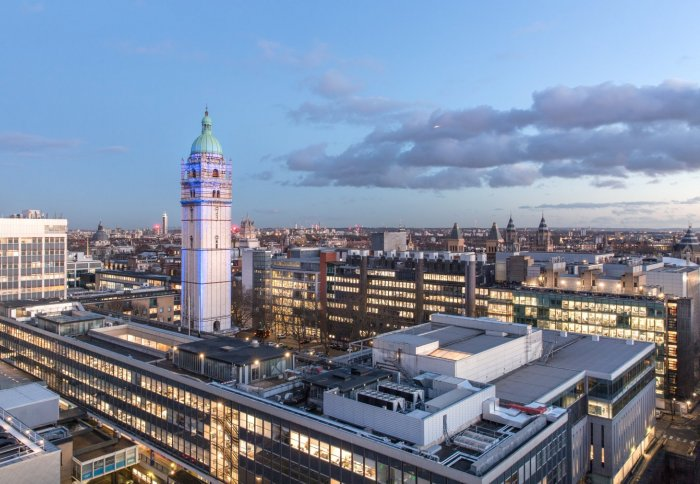
\includegraphics[width=0.8\textwidth]{Figures/imperial.jpg}
    \caption{This is an example of how you include a figure with a descriptive caption. This is an image of the South Kensington campus of Imperial College London on which we can recognize Queen's tower.}
    \label{fig:imperial-picture}
\end{figure}

Here is some filler text to show you what a few pages may look like. 
\lipsum[2-4] See Figure \ref{fig:imperial-picture}. \textbf{This is how you reference your figure in the text.}

\begin{table}[]
    \centering
    \begin{tabular}{llr}  
        \toprule
        \multicolumn{2}{c}{Module} \\
        \cmidrule(r){1-2}
        Module code    & Module name & Number of students \\
        \midrule
              & per gram    & 13.65      \\
                      &    each     & 0.01       \\
        Gnu       & stuffed     & 92.50      \\
        Emu       & stuffed     & 33.33      \\
        Armadillo & frozen      & 8.99       \\
        \bottomrule
    \end{tabular}
    \caption{Example booktabs table. Booktabs tables are nicer than regular ones. This site has a nice GUI for making LaTeX tables, and has a Booktabs option: https://www.tablesgenerator.com/}
    \label{tab:my_label}
\end{table}

\lipsum[1-4] \textbf{This is how you would reference a table:} Table \ref{tab:my_label}. 

\section{Section Example}
\label{sec:sec_example}
\lipsum[1]
\subsection{Subsection Example}
\label{sec:subsec_example}
\lipsum[1]

\subsubsection{Subsubsection Example}

Note that you can reference chapters, sections, subsections and subsubsections. For example: Subsection \ref{sec:subsec_example}!

\section{Math Example}

While math can be written inline like so $f(x) = \sum_{n=0}^{\infty} \frac{x^n}{n!}$, we often need to write stand-alone equations like so
\begin{equation}
\textrm{score}(x) = \left(\lambda_m\sum_{i=0}^{|\mathbf{m}|} \log \hat{p}_m(d(x, \mathbf{m}_i) \mid l_i)\right) + \left(\lambda_l\sum_{i=0}^{|\mathbf{l}|} \log\hat{p}_l(d(x, \mathbf{l}_i) \mid \mathbf{v}_i)\right) + \lambda_p \hat{p}_p(x)
\end{equation}

To write equations over multiple lines (like systems of equation or equations too long to fit the page), one can use the \textit{align} environment coupled to the \textit{subequations} environment like so
\begin{subequations}
\begin{align}
    \mathbb{P}(0 \leadsto -a) &= D\int_0^\infty dt\, k_r e^{-k_r t}\int_0^t d\tau\,\partial_x u \big|_{x=-a}, \\
    \mathbb{P}(0 \leadsto b) &= -D\int_0^\infty dt\, k_r e^{-k_r t}\int_0^t d\tau\,\partial_x u \big|_{x=b}.
\end{align}
\end{subequations}

\section{Algorithm Example}

See Algorithm \ref{algorithm:posit}

\begin{algorithm}[]
\SetAlgoLined
\SetKwInOut{KwInput}{Input}
\SetKwInOut{KwOutput}{Output}
\SetKwInOut{KwPre}{Pre}
\SetKw{Return}{return}
\SetKwProg{Fn}{Function}{}{end}
\LinesNumbered
\KwInput{$\textbf{m}$, such that $\mathbf{m}_i$ is the position of the $i$'th monitor\newline
$\textbf{l}$, such that $\mathbf{l}_i$ is the position of the $i$'th landmark\newline
$\mathbf{p}^m$, such that $\mathbf{p}^m_i$ is the ping latency from monitor $i$ to the target\newline
$\mathbf{p}^l$, such that $\mathbf{p}^l_i$ is the set of ping latencies to landmark $i$}

\BlankLine
\KwPre{Compute $\hat{p}_m(d \mid l)$, an estimator giving the likelihood of the target being distance $d$ away from the monitor, given that the monitor records a latency of $l$ to that target. Implemented by training a KDE using $\mathbf{p}^l$.\newline
Compute $\hat{p}_l(d \mid v)$, an estimator giving the likelihood of the target being distance $d$ away from the landmark, given a Canberra distance of $v$ between the target and the landmark, using training targets.
}
\BlankLine
\KwOutput{Most likely location of the target}
\BlankLine

\Fn{Likelihood($x$, $\mathbf{v}$)} {
MonitorScore $\gets \sum_{i=0}^{|\mathbf{m}|} \log{\hat{p}_m(d(x, \mathbf{m}_i) \mid l_i)}$\;
LandmarkScore $\gets \sum_{i=0}^{|\mathbf{l}|} \log{\hat{p}_l(d(x, \mathbf{l}_i) \mid \mathbf{v}_i)}$\;
\Return MonitorScore + LandmarkScore
}

\BlankLine
$\mathbf{v} \gets $\{$\mathrm{canberra\_distance}(\mathbf{l}_i, \mathbf{p}^m) \mid \mathbf{l}_i \in \mathbf{l}$\}

$\mathbf{C}$ $\gets$ Constraint-Based-Geolocation($\mathbf{m}$, $\mathbf{p}^m$)\;
$\mathbf{C_l}$ $\gets$ \{$m \in \mathbf{m} \mid \mathbf{C}$ contains $m\} \cup \{l \in \mathbf{l} \mid \mathbf{C}$ contains $l$\}\;
\BlankLine
\Return argmax$_{x\in \mathbf{C_l}}$ Likelihood($x$)

 \caption{Algorithm example}
 \label{algorithm:posit}
\end{algorithm}


\section{Reference Example}

Here is how you can cite papers which you have added in the \verb!/bibs/bibliography.bib! file. You can cite single references as such \cite{Einstein1905} or multiple references like so \cite{Dirac1981,Einstein1905}. Here is a reference to a website \cite{Riemann2024}.


% \appendix
% \chapter{First Appendix}

%%%%%%%%%%%%%%%%%%%%%%%%%%%%%%%%%%%%%
\bibliography{References/bibliography.bib}
%%%%%%%%%%%%%%%%%%%%%%%%%%%%%%%%%%%%%

\end{document}